\documentclass[a4paper]{article}

\usepackage{amsmath, graphicx, float, blindtext} % for dummy text
\graphicspath{ {./images/} }
\title{Metric-Predicted Variable on One or Two Groups}
\author{Shubham Gupta}

\begin{document}
\maketitle
\section{Introduction}
\begin{itemize}
    \item We have a metric predicted variable measured from two groups.
    \item \textbf{Aim}: Find out how different/same are these two measurements. 
\end{itemize}
\section{Estimating the mean and standard deviation of a normal distribution}
\begin{itemize}
    \item Normal distribution is given as:
    \[
        p(y|\mu, \sigma) = \frac{1}{Z}exp\bigg(-\frac{1}{2} \frac{(y-\mu)^2}{\sigma^2}\bigg)
    .\] 
    \[
        Z = \sigma(2\pi), \text(Z is the normalizer)
    .\] 
    \item Probability density of a dataset $D$ containing values $y_1, y_2, y_3$ is:
    \[
        p(D|\mu, \sigma)
    .\] 
    \item How to allocate probability across combinations of $\mu$ and $\sigma$?
    \[
        p(\mu, \sigma | D) = \frac{p(D|\mu, \sigma) p(\mu, \sigma)}{\int\int d\mu d\sigma p(D|\mu, \sigma) p(\mu, \sigma)}
    .\] 
    \begin{figure}[H]
        \centering
        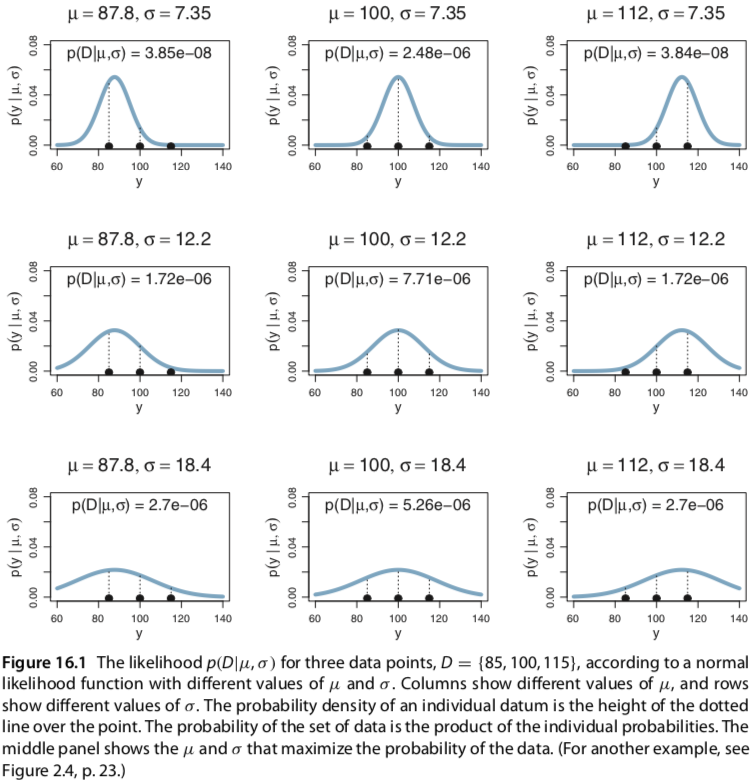
\includegraphics[width=0.8\textwidth]{mu_sigma_combinations}
        \caption{Combinations of $\mu$ and $\sigma$ for different y values}
        \label{fig:mu_sigma_combinations}
    \end{figure}
\end{itemize}
\section{The \textbf{t} distribution} 
\begin{itemize}
    \item \textbf{t} disitrbution has heavy tails. 
    \begin{figure}[H]
        \centering
        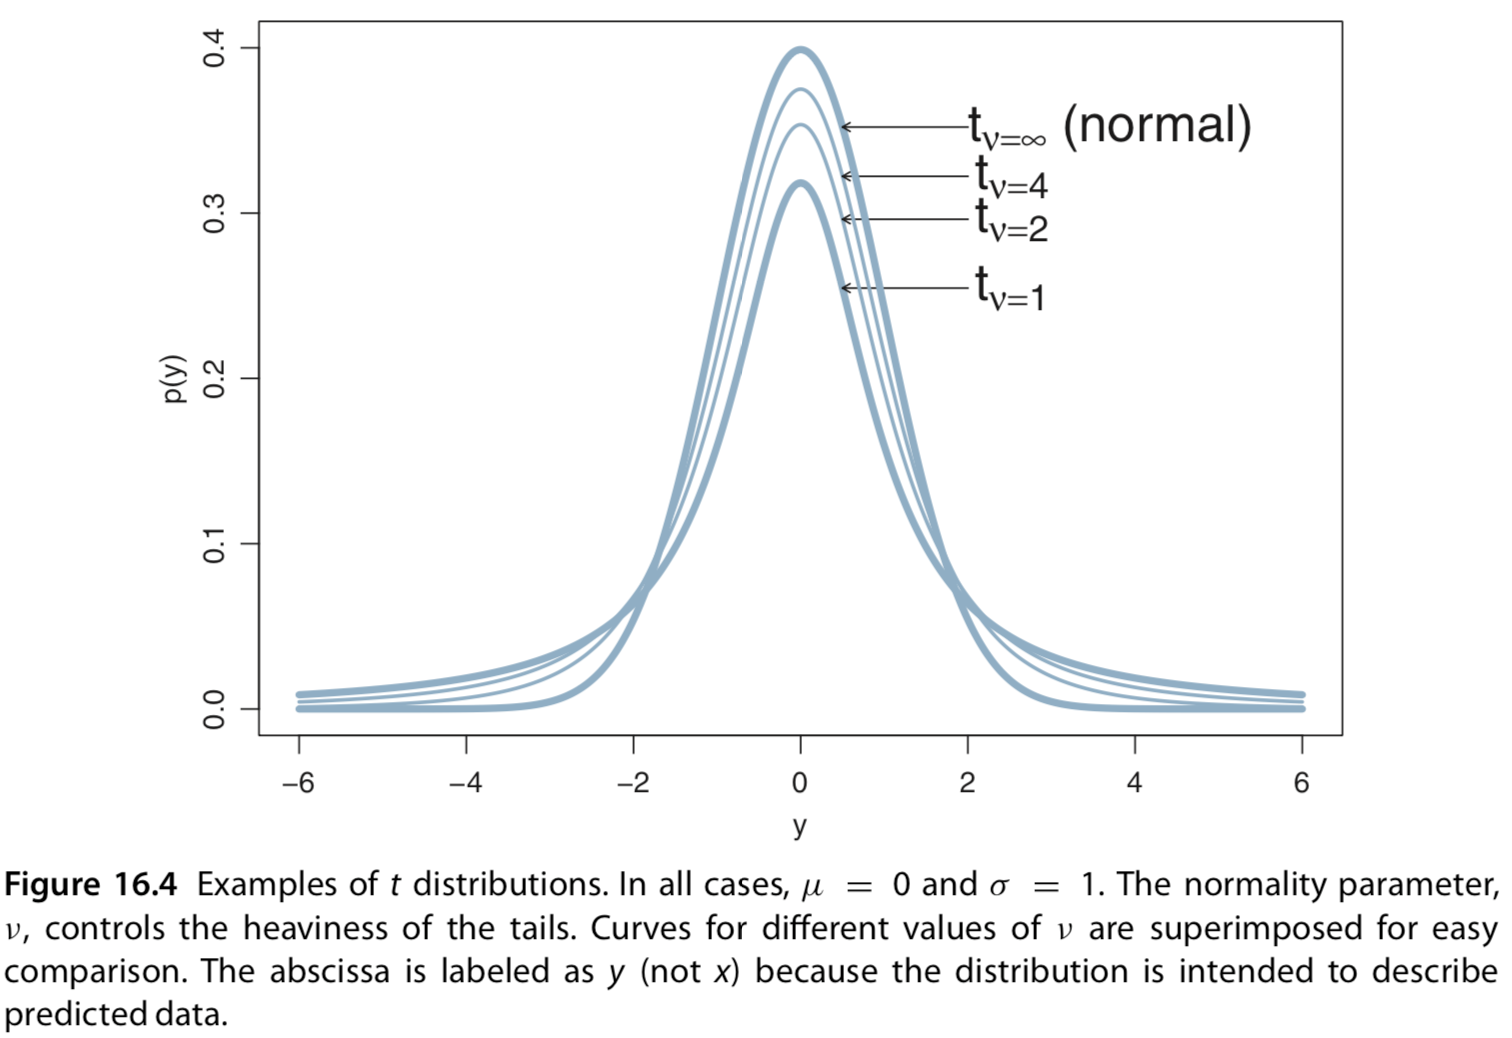
\includegraphics[width=0.8\textwidth]{t_distribution}
        \caption{Student's T disitribution}
        \label{fig:t_distribution}
    \end{figure}
    \item It has 3 parameters:
    \begin{itemize}
        \item $\mu$ controls the mean
        \item $\sigma$ controls the width
        \item $\nu$ controls heaviness of tails. Also called \textbf{normality} parameter. When $\nu = 0$, heavy tails. When $\nu = \infty$ normal distribution shape. 
        \item We will use the $t$ distribution as a descriptive model of data with outliers. $t$ distributions are robust to outliers.
        \begin{figure}[H]
            \centering
            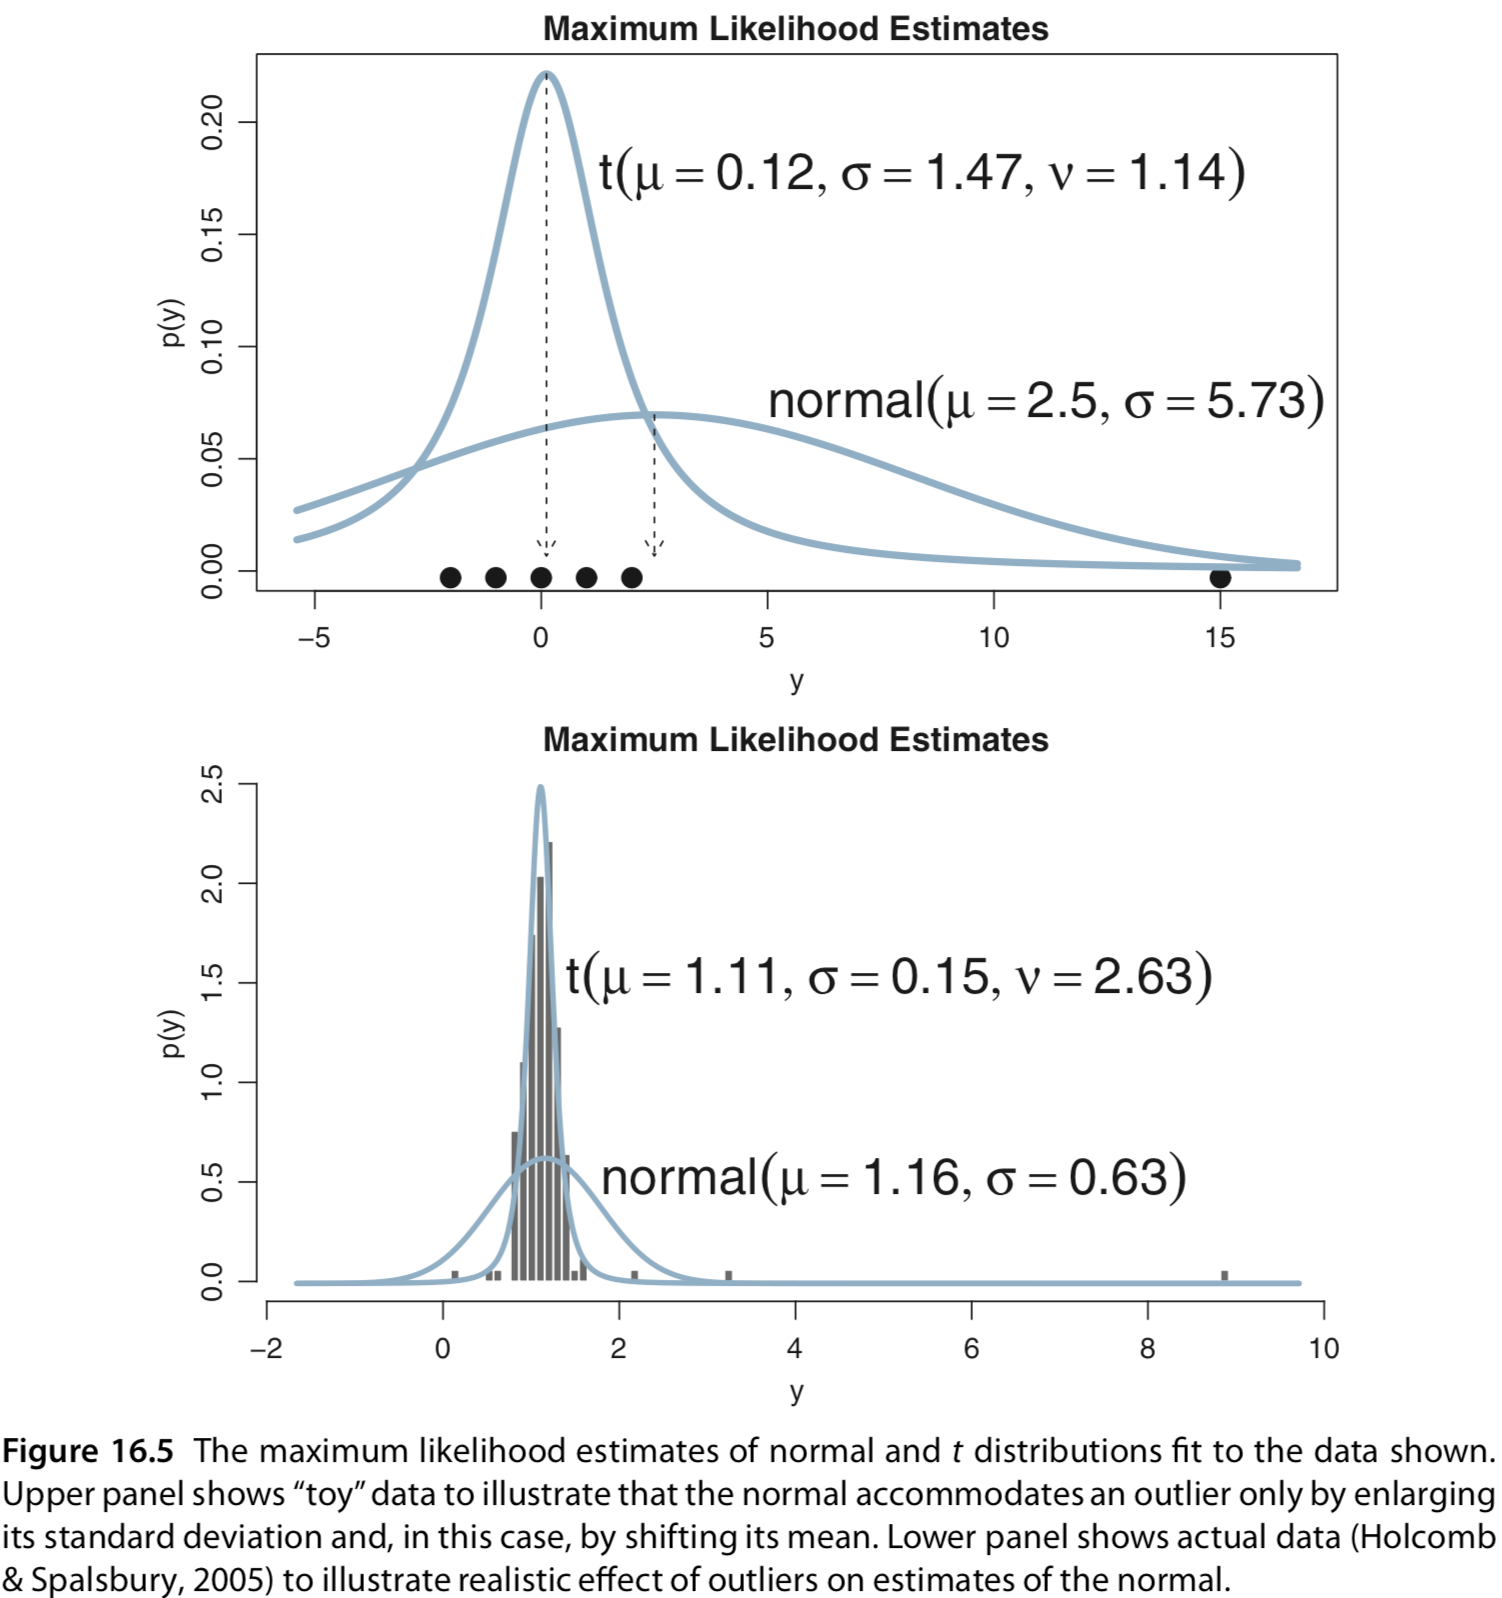
\includegraphics[width=0.8\textwidth]{t_distribution_outliers}
            \caption{MLE of t distribution and normal distributions}
            \label{fig:t_distribution_outliers}
        \end{figure}
    \item We can see that the $\mu$ for the $t$ distribution is much closer to the data points than the normal distribution. The last data point is accomodated by setting the \textbf{normality} to a \textbf{very small value}.  
    \item $\sigma$ is \textbf{not the standard deviation} for t distribution. Standard deviation will be more than $\sigma$ because of the large tails. 
    \item Use of tailed distributions is called \textbf{robust estimation} as it helps ensure our models ar erobust to outliers. 
    \item When we pick the prior distribution for $\nu$, we need to pick a distribution that gives higher chance to values under 30 and lower chance to value above 30(since above 30, t distribution will be similar to normal distribution)
    \item \textbf{Exponential distribution} is used. It has one paramter: reciprocal of it's mean. 
    \item Generally in JAGS/PyMC3, the exponential distribution will range from $0$ to $\infty$. We will add 1 to this value to make the distribution range from 1 to $\infty$ with $mean = 1 + oldmean$
    \begin{figure}[H]
        \centering
        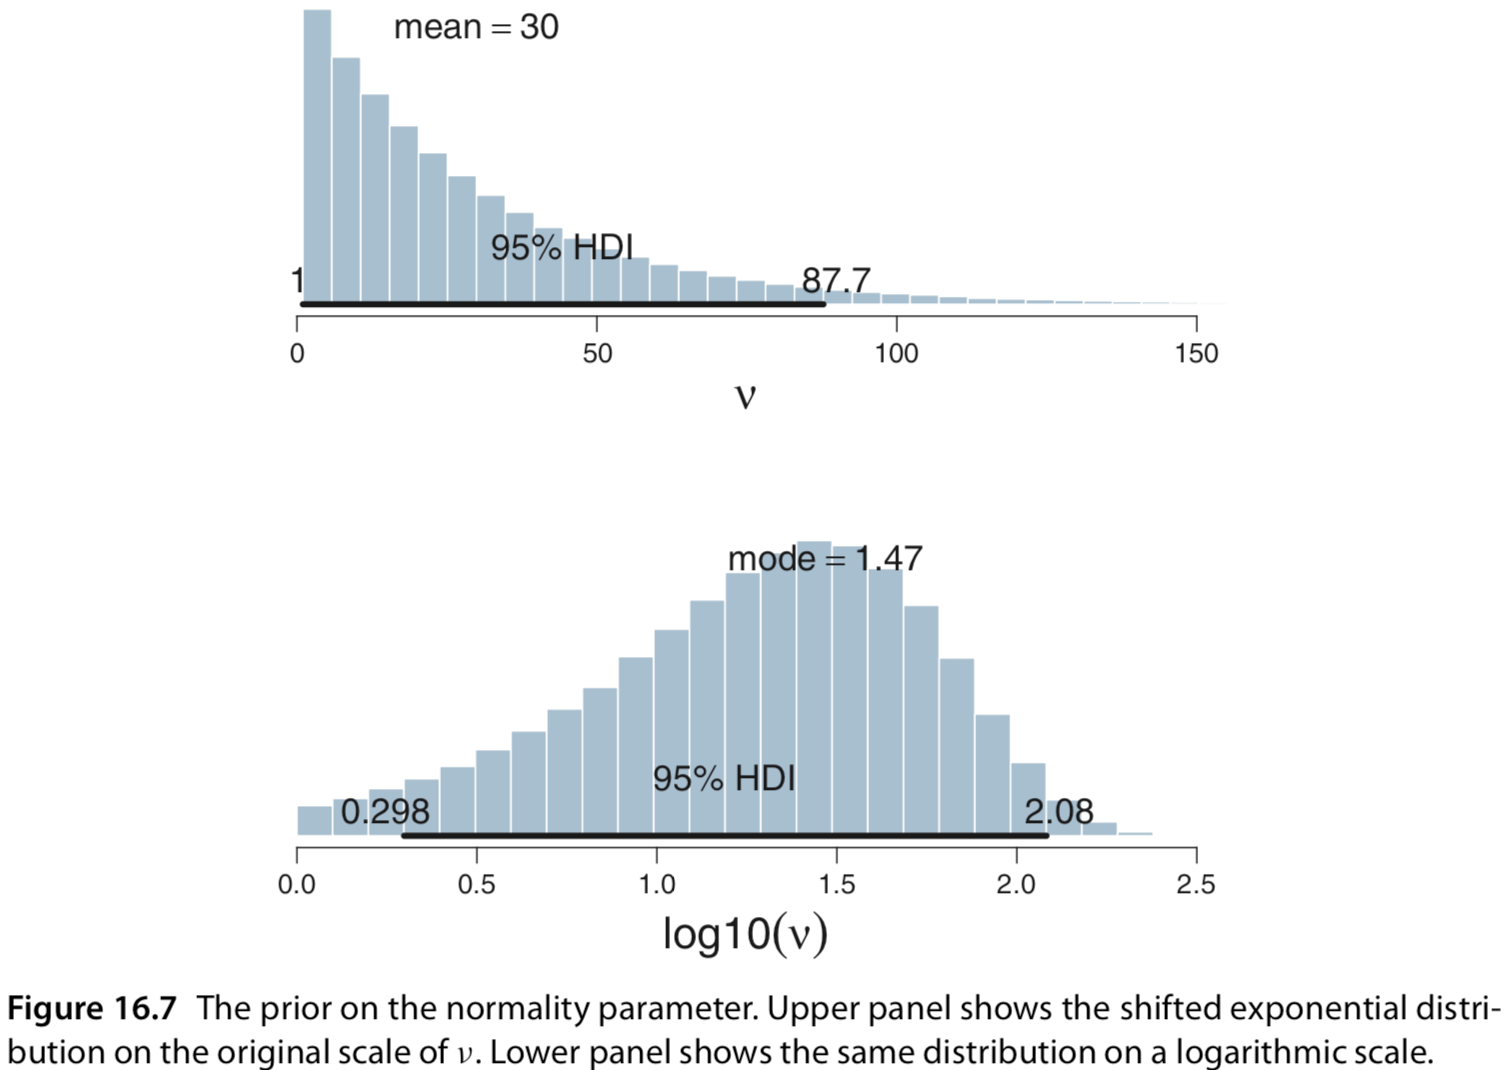
\includegraphics[width=0.8\textwidth]{normality_prior}
        \caption{Prior for nommality parameter}
        \label{fig:normality_prior}
    \end{figure}
    \item Above figure shows that the exponential distribution indeed gives more preference to values under 30.
    \begin{figure}[H]
        \centering
        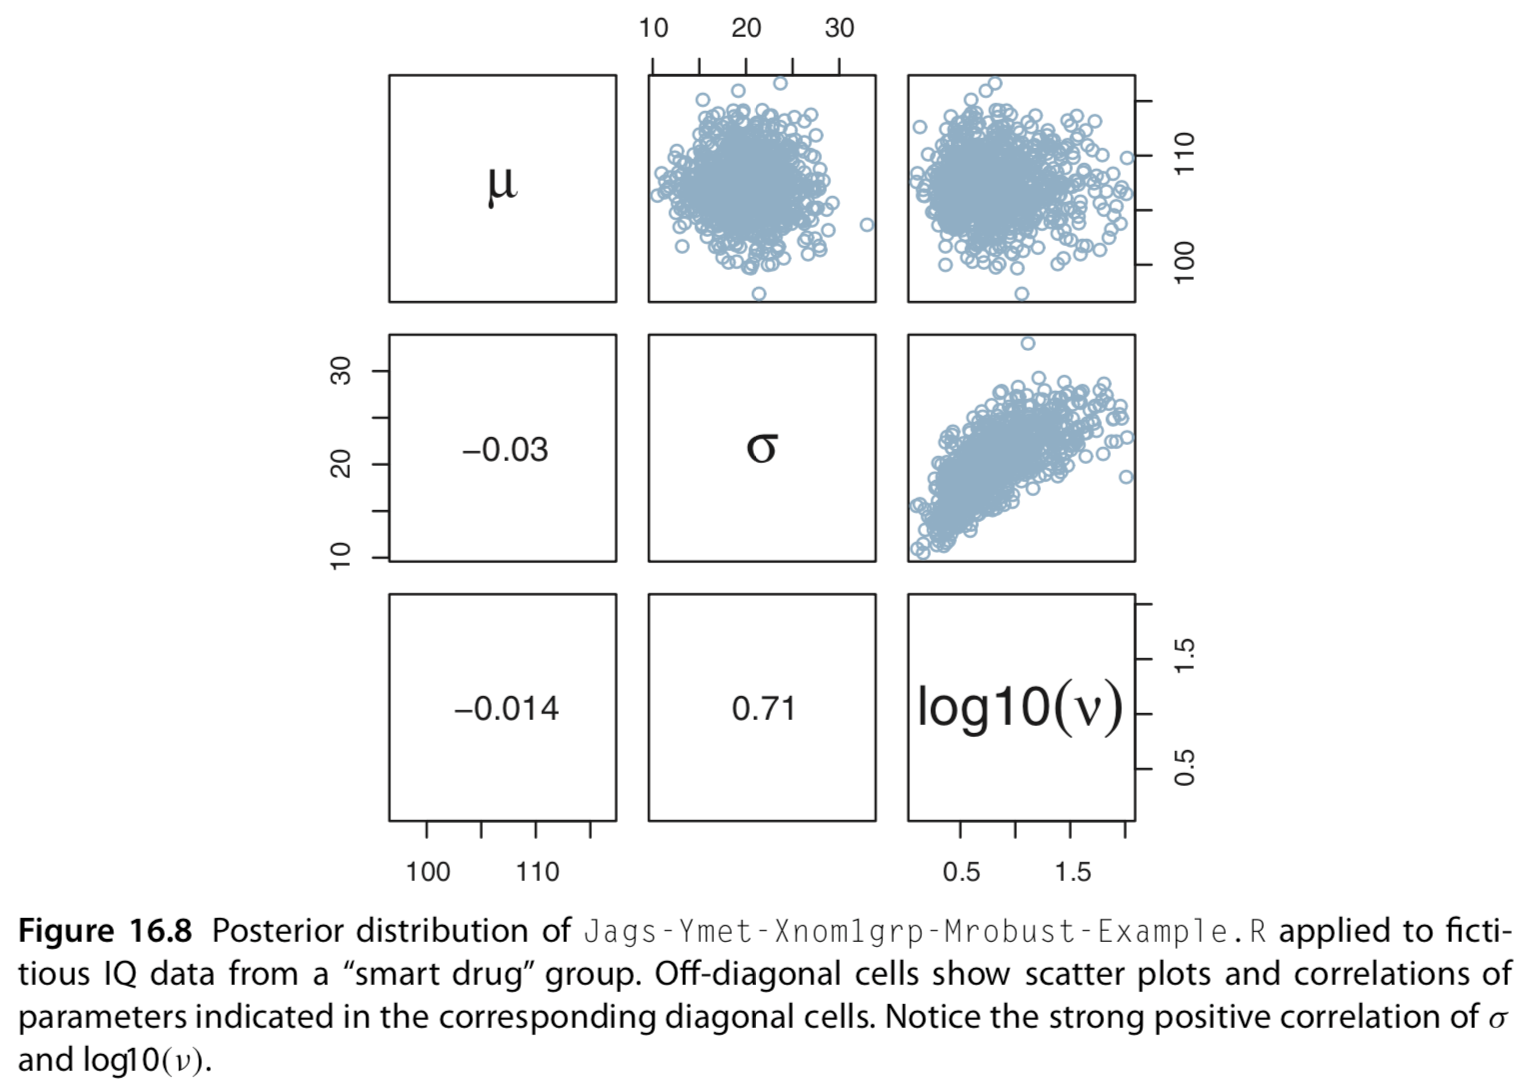
\includegraphics[width=0.8\textwidth]{inference_corelation}
        \caption{Correlation of features}
        \label{fig:inference_corelation}
    \end{figure}
    \item Above plot shows that $\nu$ is \textbf{positively} related to $\sigma$. This implies as the distribution becomes more normal, the width of the distribution also increases. This indicates that the data \textbf{contains outliers}. 
    \begin{figure}[H]
        \centering
        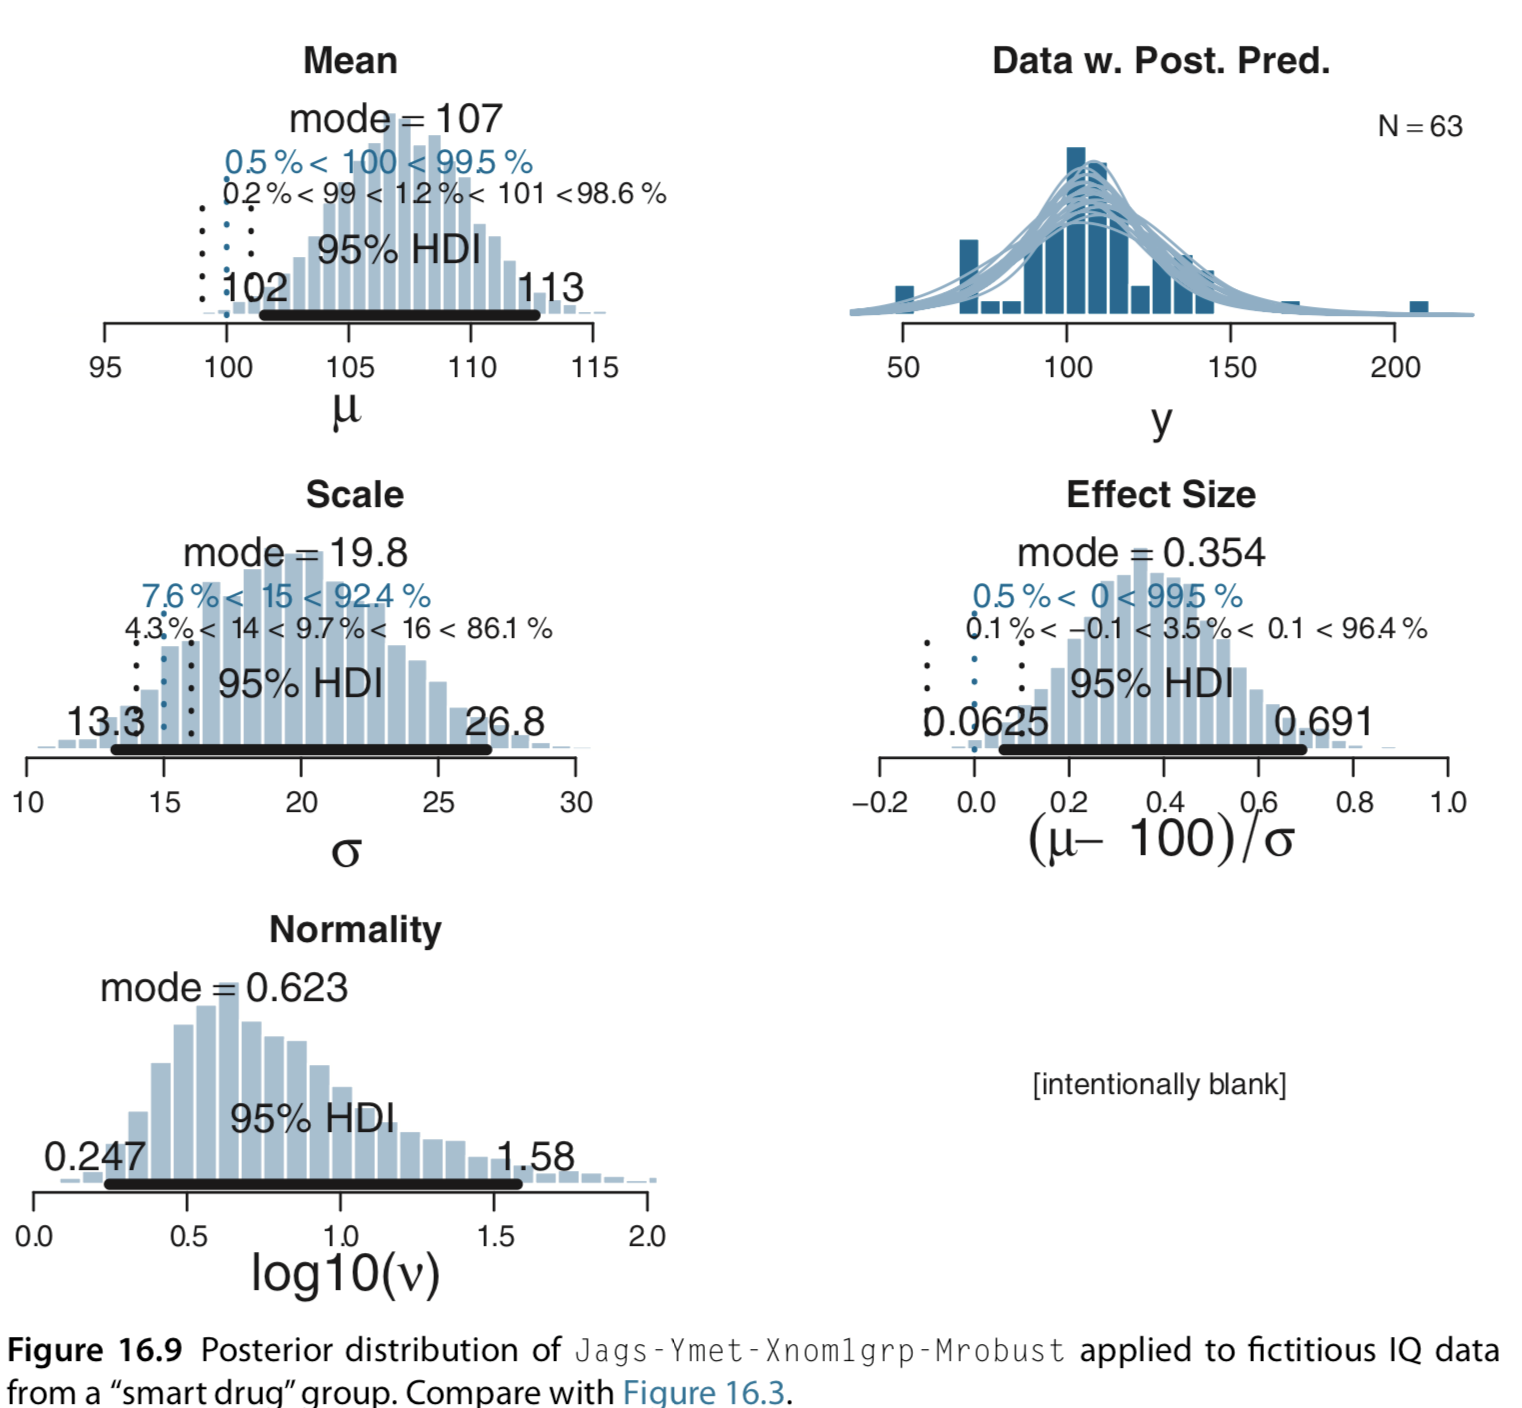
\includegraphics[width=0.8\textwidth]{posterior_distribution}
        \caption{Posterior Distribution}
        \label{fig:posterior_distribution}
    \end{figure}
\item Above plot shows that the mode for the $log_{10}\nu$ distribution is around 0.68, compared to the initial prior value. Hence, the data is better fit with smaller $\nu$ values suggesting again that there are outliers in the data.
\item For $\nu$, any value above 30 represents a near normal distribution(or above 1.47 for $log_{10}\nu$). 
    \item Upper right panel shows t-distribution can describe the data better than the normal distribution.
    \end{itemize}
\subsubsection{T-distribution in stan}
\begin{itemize}
    \item The t-distribution is represented using the $student_t(nu, mu, sigma)$.
     \item Stan model will converge faster because of the HMC method.
\end{itemize}

\subsection{Two Groups}
\begin{itemize}
    \item Generally used when we want to compare two groups.
    \item Estimate mean and scale for each group. Since there will be lesser outliers, we can use a single normaility parameter for both groups.
    \begin{figure}[H]
        \centering
        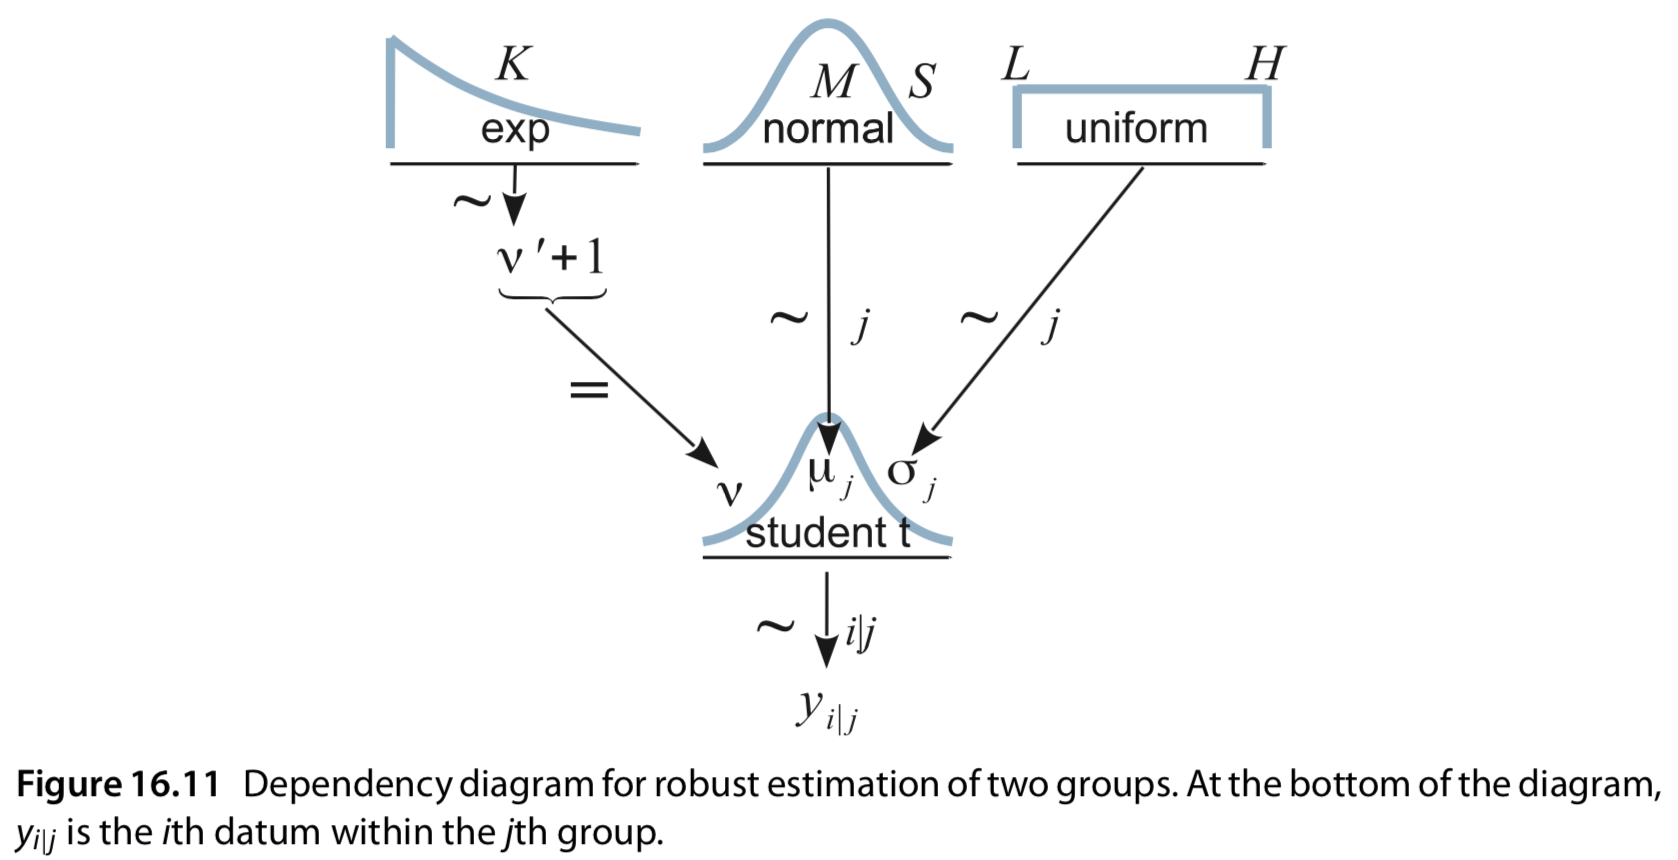
\includegraphics[width=0.8\textwidth]{two_groups_graph}
        \caption{Two groups dependency graph}
        \label{fig:two_groups_graph}
    \end{figure}
    \item We perform MCMC for the same IQ problem, and get the following:
    \begin{figure}[H]
        \centering
        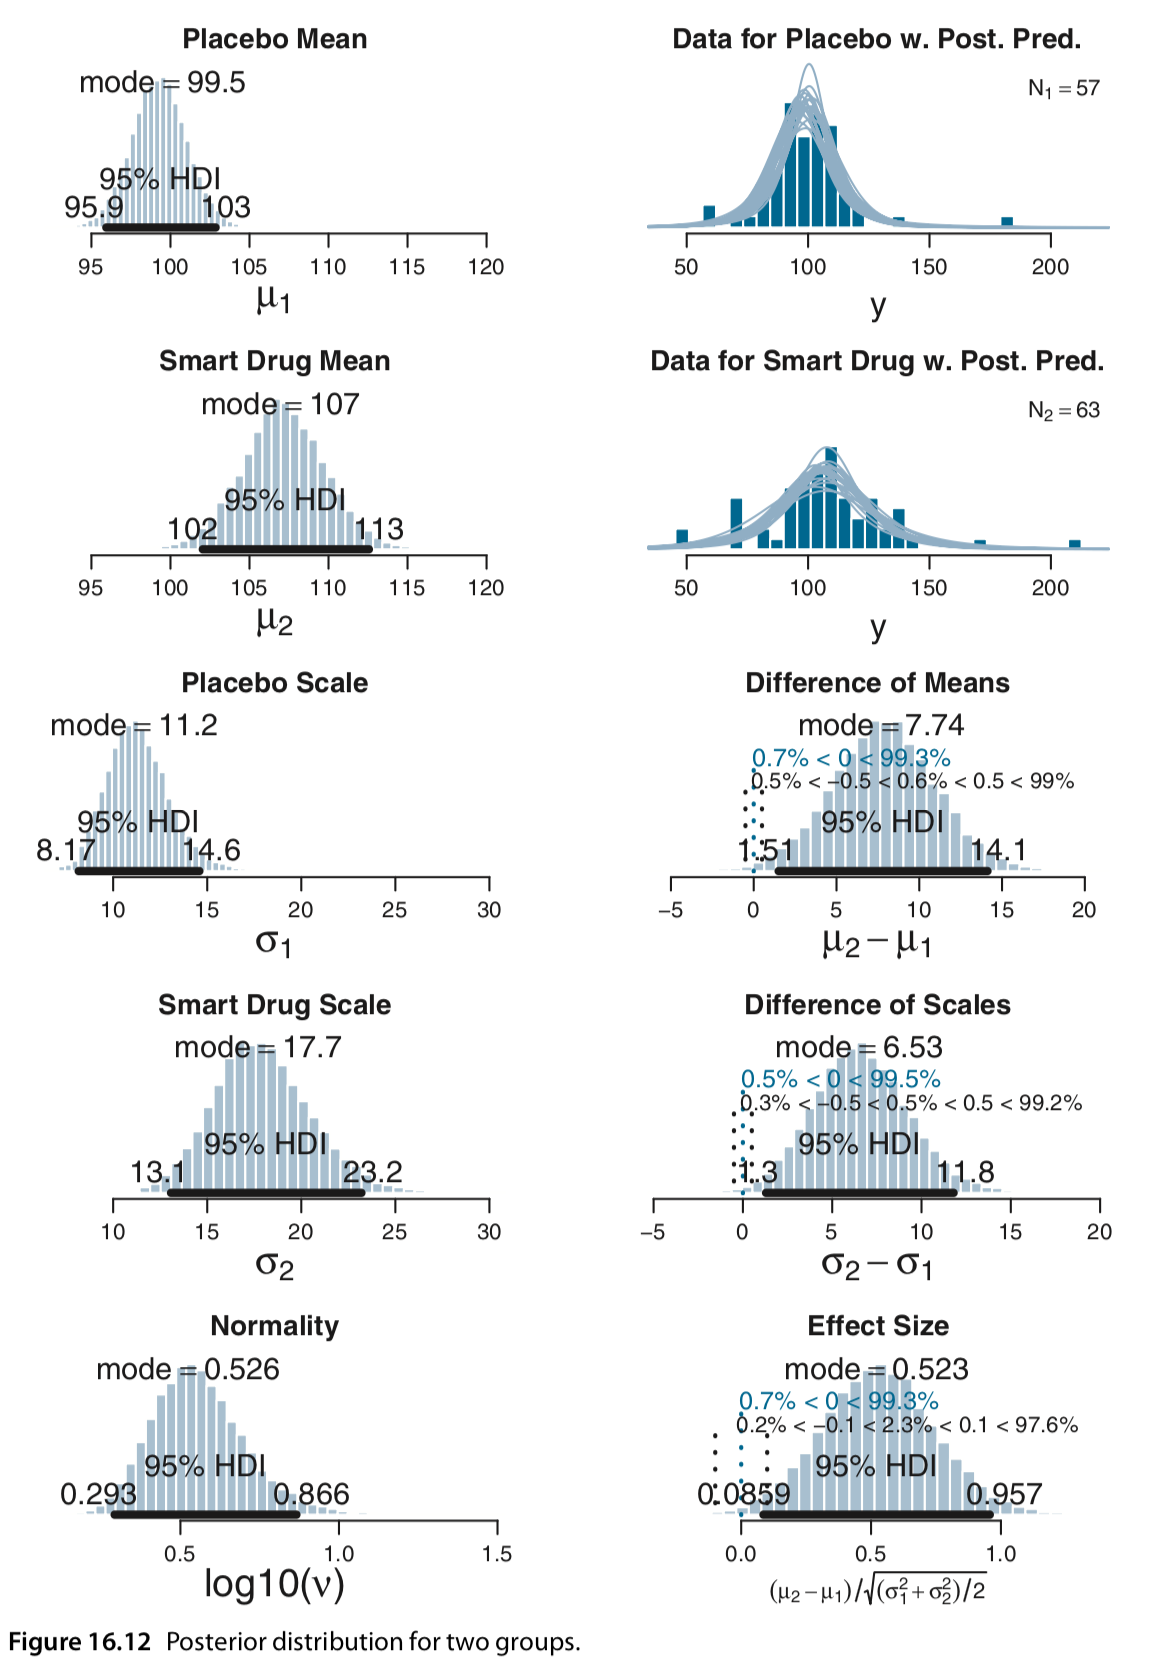
\includegraphics[width=0.8\textwidth]{two_groups_posterior}
        \caption{Two groups posterior plot}
        \label{fig:two_groups_posterior}
    \end{figure}
    \item Problems with t test:
    \begin{itemize}
        \item Provides only test of equality of means without test of equality of variances.
        \item For equality of variances, run \textbf{F Test}. But this would inflate p values for both groups. 
    \end{itemize}
\end{itemize}
\subsection{Noise Distribution}
\begin{itemize}
    \item If noise distribution does not match the data distribution, we can try the following:
        \begin{enumerate}
            \item Use better noise distribution(LOL)
            \item Transform the data so that they match the shape of the assumed noise distribution.
        \end{enumerate}
\end{itemize}
\end{itemize}
\end{document}
